%Version 3 December 2023
% See section 11 of the User Manual for version history
%
%%%%%%%%%%%%%%%%%%%%%%%%%%%%%%%%%%%%%%%%%%%%%%%%%%%%%%%%%%%%%%%%%%%%%%
%%                                                                 %%
%% Please do not use \input{...} to include other tex files.       %%
%% Submit your LaTeX manuscript as one .tex document.              %%
%%                                                                 %%
%% All additional figures and files should be attached             %%
%% separately and not embedded in the \TeX\ document itself.       %%
%%                                                                 %%
%%%%%%%%%%%%%%%%%%%%%%%%%%%%%%%%%%%%%%%%%%%%%%%%%%%%%%%%%%%%%%%%%%%%%

%%\documentclass[referee,sn-basic]{sn-jnl}% referee option is meant for double line spacing

%%=======================================================%%
%% to print line numbers in the margin use lineno option %%
%%=======================================================%%

%%\documentclass[lineno,sn-basic]{sn-jnl}% Basic Springer Nature Reference Style/Chemistry Reference Style

%%======================================================%%
%% to compile with pdflatex/xelatex use pdflatex option %%
%%======================================================%%

%%\documentclass[pdflatex,sn-basic]{sn-jnl}% Basic Springer Nature Reference Style/Chemistry Reference Style


%%Note: the following reference styles support Namedate and Numbered referencing. By default the style follows the most common style. To switch between the options you can add or remove “Numbered” in the optional parenthesis. 
%%The option is available for: sn-basic.bst, sn-vancouver.bst, sn-chicago.bst%  
 
\documentclass[pdflatex,sn-nature]{sn-jnl}% Style for submissions to Nature Portfolio journals
%%\documentclass[pdflatex,sn-basic]{sn-jnl}% Basic Springer Nature Reference Style/Chemistry Reference Style
%%\documentclass[pdflatex,sn-mathphys-num]{sn-jnl}% Math and Physical Sciences Numbered Reference Style 
%%\documentclass[pdflatex,sn-mathphys-ay]{sn-jnl}% Math and Physical Sciences Author Year Reference Style
%%\documentclass[pdflatex,sn-aps]{sn-jnl}% American Physical Society (APS) Reference Style
%%\documentclass[pdflatex,sn-vancouver,Numbered]{sn-jnl}% Vancouver Reference Style
%%\documentclass[pdflatex,sn-apa]{sn-jnl}% APA Reference Style 
%%\documentclass[pdflatex,sn-chicago]{sn-jnl}% Chicago-based Humanities Reference Style

%%%% Standard Packages
%%<additional latex packages if required can be included here>

\usepackage{graphicx}%
\usepackage{multirow}%
\usepackage{amsmath,amssymb,amsfonts}%
\usepackage{amsthm}%
\usepackage{mathrsfs}%
\usepackage[title]{appendix}%
\usepackage{xcolor}%
\usepackage{color, colortbl}
\usepackage{textcomp}%
\usepackage{manyfoot}%
\usepackage{booktabs}%
\usepackage{algorithm}%
\usepackage{algorithmicx}%
\usepackage{algpseudocode}%
\usepackage{listings}%
\usepackage{comment}
\usepackage{newtxtext,newtxmath}
\usepackage[utf8]{inputenc}
\usepackage{newfloat}

% Define a new floating environment for Extended Data Figures
\DeclareFloatingEnvironment[
fileext=loe,
placement={!ht},
name={Extended Data Fig.}
]{extfigure}
\DeclareUnicodeCharacter{2009}{\,}

%% as per the requirement new theorem styles can be included as shown below
\theoremstyle{thmstyleone}%
\newtheorem{theorem}{Theorem}%  meant for continuous numbers
%%\newtheorem{theorem}{Theorem}[section]% meant for sectionwise numbers
%% optional argument [theorem] produces theorem numbering sequence instead of independent numbers for Proposition
\newtheorem{proposition}[theorem]{Proposition}% 
%%\newtheorem{proposition}{Proposition}% to get separate numbers for theorem and proposition etc.

\theoremstyle{thmstyletwo}%
\newtheorem{example}{Example}%
\newtheorem{remark}{Remark}%

\theoremstyle{thmstylethree}%
\newtheorem{definition}{Definition}%

\raggedbottom
%%\unnumbered% uncomment this for unnumbered level heads

\begin{document}
%titulo 75 caracteres contando espacios
\title[Article Title]{Bayesian analysis reveals asymmetry in P2X2 receptor activation}
\author*[1]{\fnm{Luciano} \sur{Moffatt}}\email{lmoffatt@qi.fcen.uba.ar}
\author[2]{\fnm{Gustavo} \sur{Pierdominici-Sottile}}\email{gsottile@unq.edu.ar}
%\equalcont{These authors contributed equally to this work.}

%\author[1,2]{\fnm{Third} \sur{Author}}\email{iiiauthor@gmail.com}
%\equalcont{These authors contributed equally to this work.}

\affil*[1]{\orgdiv{Instituto de Qu\'{i}mica F\'{i}sica de los Materiales, Medio Ambiente y Energ\'{i}a}, \orgname{  Consejo Nacional de Investigaciones Científicas y T\'{e}cnicas}, \orgname{Universidad de Buenos Aires} , \city{Buenos Aires}, \postcode{1428},  \country{Argentina}}

\affil[2]{\orgdiv{Departamento de Ciencia y Tecnolog\'{i}a, 
  Consejo Nacional de Investigaciones Científicas y T\'{e}cnicas} \orgname{Universidad Nacional de Quilmes}, \orgaddress{\street{S\'{a}enz Pe\~{n}a 352}, \city{Bernal}, \postcode{B1876BXD}, \state{Buenos Aires}, \country{Argentina}}}

%\affil[3]{\orgdiv{Department}, \orgname{Organization}, \orgaddress{\street{Street}, \city{City}, \postcode{610101}, \state{State}, \country{Country}}}


\abstract{
	The activation of ligand-gated ion channels is fundamental to cellular signal transduction, influencing processes from neurotransmission to immune responses\cite{Changeux1984AcetylcholineRA,UNWIN199331, Lemoine2012,galligan2002ligand,feske2012ion}. ATP-gated P2X receptors, with their trimeric structure, provide a model system for investigating allosteric regulation\cite{Nicke1998P2X1AP,Sattler2020UnravellingTI,Hattori2012MolecularMO,Moffatt_hume}. While structural studies have defined their closed and open states\cite{abierta_p2x,cerrada_p2x}, the precise sequence of ATP-driven conformational changes and the role of subunit-specific dynamics remain unresolved. 
	Here, we demonstrate that the activation kinetics of P2X2 receptors can be accurately reproduced by an asymmetric coupling mechanism, where ATP binding drives the rotation of individual subunits and a saturating increase in conductance as the subunits undergo rotation. Using a novel Bayesian analysis tailored to time-averaged macroscopic currents, we demonstrate that ATP binding stabilizes and lowers the energetic barrier for rotation of the left subunit while minimally influencing the right subunit. A second asymmetric coupling explains the negative cooperativity in binding, with ATP binding at one site paradoxically increasing the barrier at the second site. These modulated energy barriers prevent an unliganded rotation that would lead to premature inactivation. 
	Our findings suggest that tunable activation barriers are a general strategy for stabilizing ion channels and signaling proteins in dynamic cellular environments. This framework advances our understanding of allosteric regulation in ligand-gated ion channels and may inform drug design for P2X receptors in conditions such as chronic pain and inflammation.
	}


\keywords{Bayesian Analysis, P2X receptors, Cellular Signaling}

\maketitle
\section{Introduction}

Ligand-gated ion channels (LGICs) are multimeric membrane proteins that transduce chemical signals into electrical responses by coupling ligand binding to the opening of an ion‐conducting pore \cite{Changeux1984AcetylcholineRA,UNWIN199331,Lemoine2012,galligan2002ligand,feske2012ion}. These receptors convert the energy of ligand binding into conformational changes that modulate pore conductance, thereby transforming chemical signals into electrical ones—a process underlying fast synaptic transmission \cite{nakanishi1994metabotropic,greengard2001neurobiology}, muscle contraction \cite{peper1982acetylcholine}, and other vital physiological functions \cite{burnstock2007physiology}. Among LGICs, ATP-gated P2X receptors are particularly attractive as a model system due to their trimeric architecture \cite{trimer}, intersubunit ATP-binding sites \cite{MarquezKlaka2007IdentificationOA}, and the availability of high-resolution structures for both open \cite{abierta_p2x} and closed \cite{cerrada_p2x} states.

A comprehensive understanding of P2X receptor activation requires a framework linking molecular mechanisms to the kinetic variability observed in experiments. While single-channel Markov models capture the stochastic behavior of individual channels \cite{properties_single_channe}, macroscopic current fluctuations primarily reflect the collective opening and closing of many channels \cite{Moffatt_hume}. Historically, a disconnect has persisted between kinetic schemes derived from single-channel data \cite{properties_single_channe} and the molecular mechanisms of channel activation \cite{Hattori2012MolecularMO}. The allosteric Monod–Wyman–Changeux (MWC) model \cite{Changeux1984AcetylcholineRA} has provided a thermodynamic framework to unite these aspects, as demonstrated in studies on channels such as BK \cite{Horrigan2002CouplingBV} and, more recently, purinergic receptors \cite{Moffatt_hume}.

Here, we bridge this divide with two complementary advances. First, we introduce \textit{MacroIR}, a Bayesian framework that efficiently analyzes time-averaged macroscopic currents by preserving temporal correlations and enabling rapid evaluation of complex kinetic schemes. Second, we develop conformational models that directly link kinetic transitions to physical subunit rotations—thus avoiding hypothetical states (e.g., the flip state). Together, these approaches yield robust Bayesian evidence for kinetic asymmetry in P2X2 receptor activation, redefining ligand efficacy in energetic terms and offering a blueprint for integrating kinetic data with structural mechanisms.


\section{Methods}\label{sec:methods}

We describe here the experimental data used to evaluate our approach, the kinetic schemes constructed for prediction, the likelihood function quantifying predictive accuracy, and the algorithm for determining Bayesian evidence to compare alternative kinetic schemes and infer posterior parameter distributions.

\subsection{Experimental Data: Outside-out Patch Recording}

The experimental dataset analyzed in this study was previously published in \textit{The Journal of General Physiology} \cite{Moffatt_hume} and is reexamined here to develop and validate our approach. Recordings were obtained from macro outside-out patches containing hundreds to thousands of P2X2 channels. These patches were exposed to 0.2-ms ATP pulses at concentrations of 0.2, 0.5, 1, 2, and 10 mM delivered every 2 minutes, interspersed with 10-ms pulses of 1 mM ATP. The dataset is ideally suited for kinetic analysis due to the precise alignment of stimulus timing with channel responses, which were recorded directly from the patch. For complete experimental details—including solution compositions, recording conditions, and data acquisition protocols—please refer to the original publication \cite{Moffatt_hume}.

For kinetic analysis, we segmented the data as follows. The 1-s pre-pulse period was divided into 72 intervals of equal duration. During the ATP pulse, the algorithm processed the raw data, whereas after the pulse the data were averaged over exponentially spaced intervals (approximately 10 points per decade). Additionally, for each 10-ms ATP pulse, one sample was retained from the second half of the pulse, corresponding to the equilibrium current.

\subsection{Kinetic Models Under Test}

We evaluated 11 kinetic models, including seven previously described by Moffatt and Hume \cite{Moffatt_hume} and four new models introduced in this study. These models can be classified  into three distinct categories: \textbf{state models}, which describe receptor kinetics without explicitly incorporating allosteric interactions; \textbf{allosteric models}, which introduce modulations between specific transitions without an explicit structural correspondence; and \textbf{conformational models}, which explicitly map kinetic transitions onto physical structural rearrangements.

\subsubsection{Previously Established Models}

The seven previously established models represent progressively complex descriptions of receptor activation:

\textbf{State Models:}  
- \textit{Scheme I}: A Minimal linear scheme for a homotrimeric channel in which all binding sites must be occupied before channel opening can occur.  
- \textit{Scheme II}: Extends Scheme I by introducing an intermediate "flipped" state between the fully bound and open conformations, allowing for a sequential activation process.  
- \textit{Scheme III}: Preferred scheme on a single channel study \cite{properties_single_channe}, this scheme introduces multiple open states converging into a final closed state, refining receptor deactivation pathways.  
- \textit{Scheme IV}: Builds upon Scheme III by incorporating a flipped state.  

\textbf{Allosteric Models:}  
- \textit{Scheme V}: A \textbf{Monod-Wyman-Changeux (MWC)} model for a trimeric receptor, in which ligand binding promotes a concerted gating transition through an allosteric mechanism.  
- \textit{Scheme VI}: Introduces an explicit \textbf{flipping transition} that can be allosterically modulated. In this scheme, binding increases the probability of flipping, which in turn increases the probability of opening.  
- \textit{Scheme VII}: Extends Scheme VI by allowing flipping to occur independently at each binding site, creating a highly interconnected state network in which binding, flipping, and gating are coupled.  

At the time these models were developed, it was not yet known that the ATP-binding site of P2X receptors was inter-subunit, as in Cys-loop receptors, rather than intra-subunit, as in glutamate receptors. Consequently, these models did not account for the complexity of ternary coupling. Later, the resolution of closed and open structures of zP2X4 \cite{cerrada_p2x, abierta_p2x} confirmed the inter-subunit nature of the ATP-binding site and suggested that agonist binding promotes subunit rotation, hinting at a potential structural mechanism for gating.

A major limitation of the allosteric models (Schemes VI and VII) was that they not only postulated allosteric coupling between binding and flipping (and between flipping and gating)—which could be justified if flipping were the structural mechanism transmitting binding energy to the pore—but also required a direct binding–gating interaction to achieve a good fit. The latter was harder to interpret mechanistically. 

\subsubsection{New Conformational Models}

Motivated by structural insights from P2X4, we developed four new models that replace the hypothetical "flipping" state with a well-defined \textbf{subunit rotation} and introduce allosteric interactions only where direct physical contact exists—between binding and subunit rotation. We considered three types of coupling:

- \textbf{RB (Rotation–Binding)}: Rotation of the right subunit forming the ATP-binding site.  
- \textbf{BR (Binding–Rotation)}: Binding-induced rotation of the subunit to the left of the ATP-binding site.  
- \textbf{RBR (Rotation–Binding–Rotation)}: Ternary coupling involving both subunits that form the ATP-binding site.  

The four new models are:

- \textbf{Scheme VIII}: Includes only RBR coupling, in which ATP binding promotes a concerted rotation of both subunits forming the binding site.  
- \textbf{Scheme IX}: Assumes RBR = 1 (i.e., no ternary coupling) and constrains RB = BR, implying symmetric interactions between ligand binding and subunit rotations.  
- \textbf{Scheme X}: Similar to Scheme IX but allows RB and BR to be independent, capturing possible asymmetries in the binding–rotation interactions.  
- \textbf{Scheme XI}: Incorporates all three coupling factors (RB, BR, and RBR) simultaneously, representing the most complete model of receptor activation in this framework.  

This conformational framework eliminates the need for poorly defined allosteric interactions and provides a direct mapping between kinetic parameters and structural changes observed in crystallographic studies.

\subsubsection{Conductance Parameterization}

For the best-performing conformational model (Scheme X), we hypothesized that conductance is a function of the number of rotated subunits. Instead of explicitly modeling the kinetics of a rotation–gating interaction (which would require a 48-state conformational model), we assumed that each rotated subunit stabilizes the open conformation, leading to an effective mean conductance that depends on the number of rotated subunits:

\[
i(n) = i_{\text{max}} \cdot \frac{E_n}{E_n + 1}, \quad E_n = E_0 \cdot F_g^n.
\]

Here, \( E_n \) represents the efficacy of the \( n \)-rotated state. This formulation significantly reduced the number of states while maintaining sufficient flexibility to capture conductance modulation. In addition to computational feasibility, this approach naturally accounts for the possibility that the pore lacks a strict blocking mechanism, and that its conductance is a nonlinear function of the number of rotated subunits.

\subsubsection{Kinetic and Equilibrium Allosteric Factors}

Previous studies extended the allosteric framework, typically applied to equilibrium constants, to kinetic rates \cite{Moffatt_hume}. In this work, we refine this approach by explicitly defining kinetic allosteric factors.

Consider two conformational transitions, \( g \) (gating) and \( r \) (rotation). In the absence of interaction, they are described by four independent kinetic parameters: \( b_{\text{on}}, b_{\text{off}}, r_{\text{on}}, r_{\text{off}} \). If an allosteric interaction exists between binding and rotation (BR coupling), then the kinetic parameters in the activated state become:

\[
b^*_{\text{on}}, b^*_{\text{off}}, r^*_{\text{on}}, r^*_{\text{off}}.
\]

Microscopic reversibility imposes a constraint on these parameters:

\[
b_{\text{on}} \cdot r^*_{\text{on}} \cdot b^*_{\text{off}} \cdot r_{\text{off}} = r_{\text{on}} \cdot b^*_{\text{on}} \cdot r^*_{\text{off}} \cdot b_{\text{off}},
\]

which simplifies to:

\[
\frac {\frac {b_{\text{on}}}{b_{\text{off}}}}{\frac {b^*_{\text{on}}} {b^*_{\text{off}}}} = \frac {\frac {r_{\text{on}}}{r_{\text{off}}}}{\frac {r^*_{\text{on}}} {r^*_{\text{off}}}} = BR_{\text{eq}}.
\]

Thus, only two extra parameters are needed to determine the coupled kinetic rates, defined in terms of the forward rates:

\[
BR_{b_{\text{on}}} = \frac{b^*_{\text{on}}}{b_{\text{on}}},
\]
\[
BR_{r_{\text{on}}} = \frac{r^*_{\text{on}}}{r_{\text{on}}}.
\]

For Bayesian model selection, we only used these parameters. However, for interpretative purposes, we also considered the converse coupling factors:

\[
BR_{b_{\text{off}}} = \frac{b^*_{\text{off}}}{b_{\text{off}}},
\]
\[
BR_{r_{\text{off}}} = \frac{r^*_{\text{off}}}{r_{\text{off}}}.
\]

\subsection{Likelihood function of time averaged macroscopic currents: MacroIR}
In this section we introduce our new algorithm for the determination of the likelihood of time averaged macroscopic currents. We will first ilustrate the concepts on the case we have only one channel to build from there the complex case of macrocurrents. Also, we are developing techniques that are also relevant for single channel.   

\subsubsection{Notation}
We denote specific channel states using subscripts (e.g., \( i, j \)), while superscripts (e.g., "prior", "post", "obs") are used to indicate the type of probability distribution (e.g., prior, posterior, or observed). For instance, \( p_i^{\text{prior}} \) represents the prior probability of being in state \( i \), and \( p_i^{\text{post}} \) represents the posterior probability after an observation.
\begin{comment}
	esta incompleta (me parece)
\end{comment}
\subsubsection{Markov Model of Single-Channel Behavior}

Ion channel gating is inherently stochastic. We model channel kinetics as a Markov process with a finite set of states \(k\). The state occupancy is described by the probability vector \(\boldsymbol{p}(t)\), which evolves according to
\begin{equation}
	\frac{d\boldsymbol{p}}{dt}(t) = \boldsymbol{p}(t)\cdot \boldsymbol{Q},
	\label{eq:master_equation_short}
\end{equation}
where the off-diagonal elements of \(\boldsymbol{Q}\) are the transition rates \(k_{ij}\) and the diagonal entries satisfy
\begin{equation}
	k_{ii} = -\sum_{j\neq i} k_{ij}.
	\label{eq:Q_diag_short}
\end{equation}
The solution is given by
\begin{equation}
	\boldsymbol{p}(t) = \boldsymbol{p}(0) \cdot \exp(\boldsymbol{Q}t).
	\label{eq:solution_short}
\end{equation}
Since only the current generated by each state \(\gamma_i\) is measurable, the predicted current is
\begin{equation}
	y^{\text{pred}}(t) = \boldsymbol{p}(t)\cdot \boldsymbol{\gamma}.
	\label{eq:current_pred_short}
\end{equation}
This concise formulation links the hidden Markov dynamics to the observable current.

\subsubsection{MicroR: Bayesian Model for Instantaneous Measurements}

For a single instantaneous current measurement \(y^{\text{obs}}\), we assume an initial state probability distribution \(\boldsymbol{p}^{\text{prior}}\) and Gaussian instrumental noise with variance \(\epsilon^2\). The likelihood is
\begin{equation}
	\mathcal{L} = P(y^{\text{obs}}) = \sum_i \mathcal{N}(p_i\,\gamma_i,\,\epsilon^2),
	\label{eq:single_channel_likelihood_short}
\end{equation}
where \(\mathcal{N}(\mu,\sigma^2)\) denotes the normal distribution with mean \(\mu\) and variance \(\sigma^2\). Using Bayes' rule, the posterior state probability is updated as
\begin{equation}
	p^{\text{post}}_i = \frac{p_i\,\mathcal{N}(p_i\,\gamma_i,\,\epsilon^2)}{P(y^{\text{obs}})}.
	\label{eq:single_channel_posterior_short}
\end{equation}

For successive measurements, the prior at time \(t\) is updated via the Markov process:
\begin{equation}
	\boldsymbol{p}^{\text{prior}}(t) = \boldsymbol{p}^{\text{post}}(0) \cdot \boldsymbol{P}(t),
	\label{eq:prior_update_short}
\end{equation}
with \(\boldsymbol{P}(t)=\exp(\boldsymbol{Q}t)\). The cumulative log-likelihood for a series of observations is then
\begin{equation}
	\log \mathcal{L} = \sum_n \log \mathcal{L}_n.
	\label{eq:total_loglikelihood_short}
\end{equation}


\subsubsection{MicroIR: Bayesian Model for Time-Averaged Single-Channel Measurements}

MicroIR extends classical Bayesian analysis to time-averaged measurements, offering an alternative solution to the missing events problem (see, e.g., Colquhoun \textit{et al.}). Instead of instantaneous observations, we record the time-averaged current \(\overline{y}^{\text{obs}}\) over an interval \(t\). Although the channel state fluctuates continuously during \(t\), the analysis relies solely on the initial state probability \(\boldsymbol{p}^{\text{prior}}\) and its evolution via \(\mathbf{P}(t)\) (Eq.~\ref{eq:master_equation_solution}).

The joint probability of starting in state \(i\) and ending in state \(j\) is defined as
\begin{equation}
	\Pi_{i\rightarrow j}^{\text{prior}} = p_i^{\text{prior}}\,P_{i\rightarrow j},
	\label{eq:joint_state_probability_short}
\end{equation}
or equivalently, in matrix form, \(\boldsymbol{\Pi}^{\text{prior}} = \mathrm{diag}(\boldsymbol{p}^{\text{prior}})\,\mathbf{P}\).

The likelihood of observing \(\overline{y}^{\text{obs}}\) is then given by
\begin{equation}
	\mathcal{L} = \sum_{i,j} \Pi_{i\rightarrow j}^{\text{prior}}\,\mathcal{N}\!\Bigl(\overline{y}^{\text{obs}} - \Pi_{i\rightarrow j}^{\text{prior}}\,\overline{\Gamma}_{i\rightarrow j},\, \epsilon^2 + \sigma^2_{\overline{\Gamma}_{i\rightarrow j}}\Bigr),
	\label{eq:integrated_likelihood_short}
\end{equation}
where \(\overline{\Gamma}_{i\rightarrow j}\) and \(\sigma^2_{\overline{\Gamma}_{i\rightarrow j}}\) denote the mean and variance of the current for transitions from \(i\) to \(j\).

Using Bayes' rule, the posterior joint probability becomes
\begin{equation}
	\Pi_{i\rightarrow j}^{\text{post}} = \frac{\Pi_{i\rightarrow j}^{\text{prior}}\,\mathcal{N}\!\Bigl(\overline{y}^{\text{obs}} - \Pi_{i\rightarrow j}^{\text{prior}}\,\overline{\Gamma}_{i\rightarrow j},\, \epsilon^2 + \sigma^2_{\overline{\Gamma}_{i\rightarrow j}}\Bigr)}{P(\overline{y}^{\text{obs}})}.
	\label{eq:integrated_posterior_short}
\end{equation}
Marginalization over the initial state yields the prior for the next interval:
\begin{equation}
	p_j^{\text{prior}}(t_{n+1}) = \sum_i \Pi_{i\rightarrow j}^{\text{post}}.
	\label{eq:next_prior_short}
\end{equation}
Cumulative log-likelihood is then updated additively over successive intervals. Although the exact distribution of the mean current is not strictly normal, we approximate it as such, assuming instrumental noise dominates over gating noise.

This approach, while not applied in the present work, provides a conceptual basis for MacroIR and can be generalized to other single-molecule systems, such as molecular motors.


\subsubsection{Calculation of the Average Current Conditional on Starting and Ending States}

The time-averaged current for transitions from state \(i\) to state \(j\) over an interval \(t\) is defined as
\begin{equation}
	\overline{\Gamma}_{i \rightarrow j} = \frac{1}{t\,P_{i\rightarrow j}} \int_0^t \sum_k P_{i\rightarrow k}(\tau)\,\gamma_k\,P_{k\rightarrow j}(t-\tau)\,d\tau,
	\label{eq:gamma_ij_integral_short}
\end{equation}
where \(P_{i\rightarrow j}\) is the overall transition probability and \(\gamma_k\) is the current associated with state \(k\).

Employing the spectral decomposition of the rate matrix \(\mathbf{Q}\), this expression can be recast in closed form:
\begin{equation}
	\overline{\Gamma}_{i \rightarrow j} = \frac{1}{P_{i\rightarrow j}} \sum_{k, n_1, n_2} V_{i n_1}\,V^{-1}_{n_1 k}\,\gamma_k\,V_{k n_2}\,V^{-1}_{n_2 j}\,E_2(\lambda_{n_1}t,\lambda_{n_2}t),
	\label{eq:gamma_ij_formula_short}
\end{equation}
where \(\mathbf{V}\) and \(\mathbf{V}^{-1}\) are the eigenvector matrix of \(\mathbf{Q}\) and its inverse, \(\lambda_{n}\) are the corresponding eigenvalues, and
\begin{equation}
	E_2(x,y)=
	\begin{cases}
		\frac{e^x-e^y}{x-y}, & x\neq y, \\
		e^x, & x=y.
	\end{cases}
	\label{eq:E2_short}
\end{equation}


\subsubsection{Variance of the Average Current Conditional on Starting and Ending States}

The variance of the time-averaged current for transitions from state \(i\) to \(j\) is defined as
\begin{equation}
\mathrm{Var}(\overline{\Gamma}_{i\rightarrow j}) = E\bigl[\overline{\Gamma}_{i\rightarrow j}^2\bigr] - \Bigl(E[\overline{\Gamma}_{i\rightarrow j}]\Bigr)^2,
\label{eq:variance_gamma_short}
	\end{equation}
	with \(E[\overline{\Gamma}_{i\rightarrow j}]\) given by Eq.~\ref{eq:gamma_ij_integral}.

The expected square of the average current is initially written as
\begin{equation}
E\bigl[\overline{\Gamma}_{i\rightarrow j}^2\bigr] = \frac{1}{t^2\,P_{i\rightarrow j}} \int_0^t\int_0^{t-\tau_1} \sum_{k_1,k_2} P_{i\rightarrow k_1}(\tau_1)\,\gamma_{k_1}\,P_{k_1\rightarrow k_2}(\tau_2)\,\gamma_{k_2}\,P_{k_2\rightarrow j}(t-\tau_1-\tau_2)\,d\tau_1\,d\tau_2.
\label{eq:expected_square_integral_short}
\end{equation}

Using the spectral decomposition of \(\mathbf{Q}\), a closed-form expression is obtained:
	\begin{equation}
	E\bigl[\overline{\Gamma}_{i\rightarrow j}^2\bigr] = \frac{1}{P_{i\rightarrow j}} \sum_{k_1,k_2,n_1,n_2,n_3} V_{i n_1}\,V^{-1}_{n_1 k_1}\,\gamma_{k_1}\,V_{k_1 n_2}\,V^{-1}_{n_2 k_2}\,\gamma_{k_2}\,V_{k_2 n_3}\,V^{-1}_{n_3 j}\,E_3(\lambda_{n_1}t,\lambda_{n_2}t,\lambda_{n_3}t),
\label{eq:expected_square_closed_short}
\end{equation}
where the auxiliary function \(E_3\) is defined as
\begin{equation}
E_3(x,y,z)= 
\begin{cases}
E_{111}(x,y,z), & x\neq y,\; y\neq z,\; z\neq x,\\[1mm]
E_{12}(x,y),   & x\neq y,\; x\neq z,\; y=z,\\[1mm]
	E_{12}(y,z),   & y\neq z,\; y\neq x,\; z=x,\\[1mm]
	E_{12}(z,x),   & z\neq x,\; z\neq y,\; x=y,\\[1mm]
\frac{1}{2}e^x, & x=y=z.
\end{cases}
\label{eq:E3_short}
\end{equation}
Here,
	\begin{equation}
	E_{12}(x,y)= E_{1,11}(x,y,y) + \frac{e^y}{y-x}\Bigl(\frac{y-x-1}{y-x}\Bigr),
		\label{eq:E12_short}
		\end{equation}
		and
		\begin{equation}
		E_{1,11}(x,y,z)= \frac{e^x}{(x-y)(x-z)}.
	\label{eq:E1_11_short}
	\end{equation}
\subsubsection{From Single-Channel to Ensemble Channel Analysis}

For an ensemble of ion channels, the state probability vector initially yields a multinomial distribution for the state counts. However, measuring the total current refines the posterior distribution and introduces inverse correlations among states generating the same current. A detailed but computationally intensive method—the \textit{Microscopic Recursive Algorithm} (Moffatt, 2007)—constructs an ensemble state vector by applying Bayes’ rule to every possible state count. For larger systems, we adopt a more efficient \textit{Macroscopic Approach} that approximates the state distribution with a multivariate normal, using the covariance matrix to capture the observation-induced correlations.
\subsubsection{MacroR: Bayesian Framework for Instantaneous Channel Ensemble Measurements}

In the \textit{MacroR algorithm}, we treat measurements as instantaneous, focusing on the ensemble's state via its mean probability vector and covariance matrix. This approach—equivalent to a Kalman filter—yields the likelihood
\begin{equation}
\mathcal{L} = \mathcal{N}\Bigl( y^{\text{obs}} - y^{\text{pred}},\, \sigma^2_{y^{\text{pred}}} \Bigr),
\label{eq:macro_likelihood}
\end{equation}
with the predicted current
	\begin{equation}
	y^{\text{pred}} = N_{\text{ch}}\, \boldsymbol{\mu}^{\text{prior}}\, \boldsymbol{\gamma},
\label{eq:macro_predicted_y}
\end{equation}
and variance
\begin{equation}
\sigma^2_{y^{\text{pred}}} = \epsilon^2 + N_{\text{ch}}\, \boldsymbol{\gamma}^{\mathrm{T}}\, \boldsymbol{\Sigma}^{\text{prior}}\, \boldsymbol{\gamma}.
	\label{eq:macro_sigma_pred}
	\end{equation}
The posterior mean and covariance are updated as
\begin{equation}
\boldsymbol{\mu}^{\text{post}} = \boldsymbol{\mu}^{\text{prior}} + \frac{y^{\text{obs}} - y^{\text{pred}}}{\sigma^2_{y^{\text{pred}}}}\, \boldsymbol{\gamma}^{\mathrm{T}}\, \boldsymbol{\Sigma}^{\text{prior}},
\label{eq:macro_mean_posterior}
\end{equation}
	\begin{equation}
	\boldsymbol{\Sigma}^{\text{post}} = \boldsymbol{\Sigma}^{\text{prior}} - \frac{N}{\sigma^2_{y^{\text{pred}}}}\, \boldsymbol{\Sigma}^{\text{prior}}\, \boldsymbol{\gamma}\, \boldsymbol{\gamma}^{\mathrm{T}}\, \boldsymbol{\Sigma}^{\text{prior}}.
\label{eq:macro_cov_posterior}
\end{equation}
Propagation to the next time point is given by
\begin{equation}
\boldsymbol{\mu}^{\text{prior}}(t_{n+1}) = \boldsymbol{\mu}^{\text{post}}(t_n)\, \mathbf{P}(\Delta t_n),
	\label{eq:macro_mean_next_prior}
	\end{equation}
\begin{equation}
\boldsymbol{\Sigma}^{\text{prior}}(t_{n+1}) = \mathrm{diag}\Bigl(\boldsymbol{\mu}^{\text{prior}}(t_{n+1})\Bigr) + \mathbf{P}(\Delta t_n)^{\mathrm{T}} \Bigl( \boldsymbol{\Sigma}^{\text{post}}(t_n) - \boldsymbol{\mu}^{\text{post}}(t_n) \Bigr) \mathbf{P}(\Delta t_n).
\label{eq:macro_mean_next_cov}
\end{equation}
\subsubsection{MacroIR: A Bayesian Framework for Interval-Averaged Analysis of Channel Ensembles}

We introduce MacroIR (Macroscopic Interval Recursive), a Bayesian framework for analyzing time-averaged Markovian processes over successive intervals—as encountered in macropatch recordings. MacroIR leverages the \textbf{boundary state}, which represents the joint probability of starting in state \(i_0\) and ending in state \(i_t\) over an interval \([0,t]\), without explicitly expanding the state space.

The boundary state prior mean is defined as:
\begin{equation}
	(\mu^{\text{prior}}_{0 \rightarrow t})_{(i_0 \rightarrow i_t)} = (\mu^{\text{prior}})_{i_0} \, P_{i_0 \rightarrow i_t}(t),
	\label{eq:boundary_mean_prior}
\end{equation}
with the corresponding covariance:
\begin{multline}
	(\Sigma^{\text{prior}}_{0 \rightarrow t})_{(i_0 \rightarrow i_t)(j_0 \rightarrow j_t)} = P_{i_0 \rightarrow i_t}\Bigl[(\Sigma^{\text{prior}}_0)_{i_0,j_0} - \delta_{i_0,j_0}\, (\mu^{\text{prior}}_0)_{i_0}\Bigr] P_{j_0 \rightarrow j_t} \\
	+ \delta_{i_0,j_0}\,\delta_{i_t,j_t}\, (\mu^{\text{prior}}_0)_{i_0}\, P_{i_0 \rightarrow i_t}.
	\label{eq:boundary_covariance_prior}
\end{multline}

The predicted average current over the interval is given by
\begin{equation}
	\overline{y}^{\text{pred}}_{0,t} = N_{\text{ch}} \cdot \mathbf{\mu}^{\text{prior}}_{0} \cdot \overline{\gamma}_{0},
	\label{eq:macro_interval_predicted_y}
\end{equation}
where the marginalized current per state is
\begin{equation}
	(\overline{\gamma}_{0})_i = \sum_j (\overline{\Gamma})_{i \rightarrow j}.
\end{equation}

The variance of the predicted current is:
\begin{equation}
	\sigma^2_{\overline{y}^{\text{pred}}_{0 \rightarrow t}} = \epsilon^2_{0 \rightarrow t} + N_{\text{ch}} \cdot \widetilde{\mathbf{\gamma}^{\mathrm{T}} \mathbf{\Sigma}\mathbf{\gamma}} + N_{\text{ch}} \cdot \mathbf{\mu}^{\text{prior}}_{0} \cdot \sigma^2_{\overline{\gamma}_{0}},
	\label{eq:macro_interval_sigma_pred}
\end{equation}
with
\begin{equation}
	(\sigma^2_{\overline{\gamma}_{0}})_i = \sum_j (\sigma^2\,\overline{\Gamma})_{i \rightarrow j}.
\end{equation}

The effective term \( \widetilde{\mathbf{\gamma}^{\mathrm{T}} \mathbf{\Sigma}\mathbf{\gamma}} \) is computed as:
\begin{multline}
	\widetilde{\mathbf{\gamma}^{\mathrm{T}} \mathbf{\Sigma}\mathbf{\gamma}} = \mathbf{\gamma}^{\mathrm{T}}_{0 \rightarrow t} \cdot \mathbf{\Sigma}^{\text{prior}}_{0 \rightarrow t} \cdot \mathbf{\gamma}_{0 \rightarrow t} = \\
	\overline{\mathbf{\gamma}}_{0}^{\mathrm{T}} \cdot \Bigl( \mathbf{\Sigma}^{\text{prior}}_{0} - \mathrm{diag}(\mathbf{\mu}^{\text{prior}}_0) \Bigr) \cdot \overline{\mathbf{\gamma}}_{0 \rightarrow t} \\
	\quad + \mathbf{\mu}^{\text{prior}}_0 \cdot \Bigl( \overline{\mathbf{\Gamma}}_{0 \rightarrow t} \circ \overline{\mathbf{\Gamma}}_{0 \rightarrow t} \circ \mathbf{P} \Bigr) \cdot \mathbf{1},
	\label{eq:simplified_boundary_state}
\end{multline}
where \( \circ \) denotes the element-wise (Hadamard) product and \( \mathbf{1} \) is a vector of ones.

Posterior updates are performed without explicitly computing the boundary state. The posterior mean is updated as:
\begin{equation}
	\mathbf{\mu}^{\text{post}}_{0 \rightarrow t} = \mathbf{\mu}^{\text{prior}}_{0 \rightarrow t} + \frac{y^{\text{obs}}_{0 \rightarrow t} - y^{\text{pred}}_{0 \rightarrow t}}{\sigma^2_{\overline{y}^{\text{pred}}_{0 \rightarrow t}}} \cdot \widetilde{\boldsymbol{\gamma}^{\mathrm{T}} \boldsymbol{\Sigma}},
	\label{eq:macro_interval_posterior_mean}
\end{equation}
with
\begin{equation}
	\widetilde{\boldsymbol{\gamma}^{\mathrm{T}} \boldsymbol{\Sigma}} = \mathbf{1}_0^{\mathrm{T}} \cdot \mathbf{\gamma}^{\mathrm{T}}_{0 \rightarrow t} \cdot \mathbf{\Sigma}^{\text{prior}}_{0 \rightarrow t}.
	\label{eq:interval_gamma_sigma}
\end{equation}

Finally, the prior covariance for the next interval is updated by marginalizing over the initial states:
\begin{multline}
	\boldsymbol{\Sigma}^{\text{prior}}_{t} = \mathbf{P}^{\mathrm{T}} \Bigl( \boldsymbol{\Sigma}^{\text{prior}}_{0} - \mathrm{diag}(\boldsymbol{\mu}^{\text{prior}}_{0}) \Bigr) \mathbf{P} + \mathrm{diag}(\boldsymbol{\mu}^{\text{prior}}_{0} \cdot \mathbf{P}) \\
	- \frac{N}{\sigma^2_{\overline{y}^{\text{pred}}_{0 \rightarrow t}}} \, \widetilde{\boldsymbol{\gamma}^{\mathrm{T}} \boldsymbol{\Sigma}}^{\mathrm{T}} \cdot \widetilde{\boldsymbol{\gamma}^{\mathrm{T}} \boldsymbol{\Sigma}}.
	\label{eq:prior_covariance_update_0_t}
\end{multline}

In summary, MacroIR provides a recursive Bayesian framework for interval-averaged measurements, efficiently computing likelihoods and posterior distributions while circumventing the computational burden of explicit boundary state calculations.
\subsection{Model Comparison Framework}
We analyzed 11 alternative kinetic schemes representing distinct hypotheses of P2X2 activation. Bayesian evidence for each scheme was calculated using a parallel-tempering affine-invariant MCMC algorithm, which efficiently sampled high-dimensional posterior distributions. This method provided robust evidence values while mitigating the risk of sampling biases. 


\section{Bayesian Selection of Kinetic Schemes for Purinergic Receptor Activation}

To elucidate the mechanism underlying purinergic receptor activation, we employed a Bayesian framework to compare 11 alternative kinetic schemes using outside‐out patch recordings of rP2X2 receptors expressed in HEK 293 cells. Data analyzed in this study derive from our previous work \cite{Moffatt_hume}, comprising a unique dataset of macroscopic current responses to 0.2\,ms ATP pulses at concentrations ranging from 0.1 to 10\,mM, interspersed with 10\,ms pulses of 1\,mM MgATP. Bayesian evidence for each scheme was computed via affine-invariant parallel tempering, with the likelihood approximated using either the recursive MacroIR or its non-recursive variant MacroINR.

For clarity, kinetic models are classified into three categories: \textbf{state models} describe channel kinetics solely in terms of state transitions; \textbf{allosteric models} incorporate modulatory interactions without specifying the structural basis; and \textbf{conformational models} map these interactions onto explicit structural changes.

Figure \ref{fig:figure1} displays Bayesian evidence for selected schemes—two allosteric models (Fig. \ref{fig:figure1}c) and one state model (Fig. \ref{fig:figure1}b)—along with three new conformational models inspired by structural insights from P2X4 (Fig. \ref{fig:figure1}a). In the new conformational models, ATP binding at intersubunit interfaces drives receptor activation through independent rotational movements of each subunit, with distinct left and right secondary couplings mediating allosteric signaling and channel conductance determined by the number of rotated subunits.

Within this framework, we derived four conformational variants (Fig. \ref{fig:figure1}a): Scheme~X features distinct left and right couplings; Scheme~IX employs symmetric couplings; Scheme~VIII (Extended Data Fig. \ref{extfig:1}a) introduces a ternary coupling mechanism (involving left rotation, binding, and right rotation); and Scheme~XI combines independent and ternary interactions. In the ternary paradigm, modulation requires the presence of any two of the three conformational changes, favoring a concerted opening mechanism.

In parallel, we evaluated a state model, Scheme~IV (Fig. \ref{fig:figure1}b), which incorporates an intermediate flip state into a previously preferred single-channel scheme. This model comprises closed states with 0–4 bound ATP molecules, a flip state bifurcating into two open states, and a final closed state—capturing both activation and deactivation dynamics. Two allosteric models, Schemes~VI and VII (Fig. \ref{fig:figure1}c) extend this framework by coupling binding, flipping, and gating transitions; Scheme~VI assumes concerted flipping, whereas Scheme~VII allows subunit-specific flipping.

Model performance was assessed using two likelihood approximations: MacroIR, a recursive macroscopic interval integration method that accounts for temporal correlations (Fig. \ref{fig:figure1}d), and MacroINR, its non-recursive variant (Fig. \ref{fig:figure1}e). Notably, the non-recursive approach produced a different evidence ranking, underscoring its limitations.

Among the tested models, Scheme~X—featuring independent left and right couplings—achieved the highest Bayesian evidence, closely followed by Scheme~VI (Fig. \ref{fig:figure1}d). A pronounced evidence gap between Scheme~X and Schemes~IX and XI highlights the preference for independent secondary couplings over ternary interactions. Additionally, the evidence for Scheme~VII (with an expanded state space of approximately 40 states) could not be reliably estimated using MacroINR within available computational time, while Scheme~IV exhibited markedly lower evidence under the recursive method despite appearing more favorable under the non-recursive analysis.

Extended Data Fig.~\ref{extfig:1} presents an analysis of five additional schemes: three state models (Schemes~I, II, and III) (Extended Data Fig. \ref{extfig:1}b), one allosteric model (Scheme~V)(Extended Data Fig. \ref{extfig:1}c), and one conformational model (Scheme~VIII)(Extended Data Fig. \ref{extfig:1}a). Comparisons (Extended Data Fig. \ref{extfig:1}d) reveal that incorporating a flip state substantially enhances performance and that complex kinetic schemes outperform simpler models featuring a single open state. Moreover, a model relying solely on ternary coupling (Scheme~VIII) underperforms relative to Schemes~X and XI.

Collectively, these findings support a four-part hypothesis: (i) individual subunit rotation is feasible; (ii) ATP binding is allosterically coupled to the rotation of both left and right subunits; (iii) these couplings differ in magnitude; and (iv) channel conductance depends on the number of rotated subunits. This framework accounts for P2X2 activation kinetics without invoking an additional, difficult-to-justify binding–gating interaction, thereby reinforcing the validity of conformational models. We further interpret the flip state as the kinetic manifestation of individual subunit rotation.
\begin{figure}[t]
	\centering
	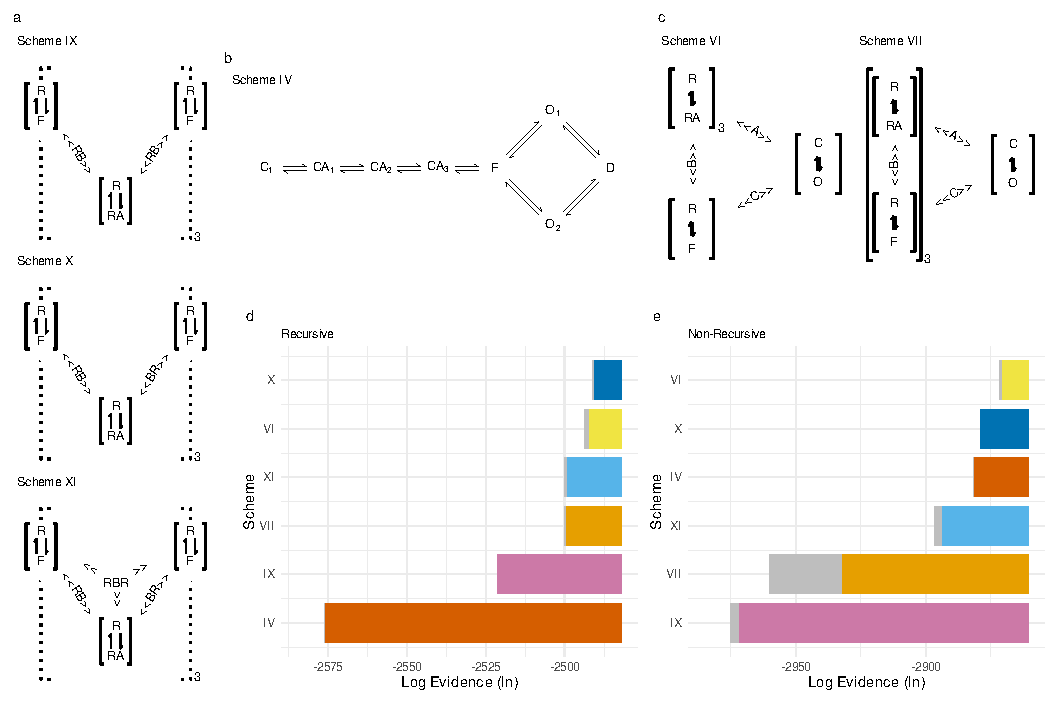
\includegraphics[width=\linewidth]{Figure_1.pdf}
	\caption{\textbf{Bayesian Evidence for Conformational, Allosteric, and State models.}  
		(\textbf{a}) Schematic representation of the newly proposed Conformational models. R: resting; F: flipped; RA: agonist-bound; RB, BR: rotation-binding and binding-rotation allosteric couplings, indicating interactions with the left or right subunit; RBR: rotation-binding-rotation ternary allosteric coupling. Dotted lines indicate sections that are repeated three times, as specified by the subscript. In Scheme~IX, RB is equal to BR, in Scheme~X they differ, and in Scheme~XI ternary coupling is also present.  
		(\textbf{b}) State Scheme~IV. C: closed state; CA$_n$: closed state with $n$ agonists bound; F: flipped state; O$_n$: $n$th alternative open state; D: a potentially desensitized closed state where unbinding is restricted.  
		(\textbf{c}) Allosteric Schemes~VI and VII. C: closed channel; O: open channel; A, B, C: allosteric couplings; subscripts indicate the number of repetitions.  
		(\textbf{d--e}) Bayesian evidence for each illustrated scheme, computed using the recursive MacroIR algorithm (\textbf{d}) and the non-recursive MacroINR algorithm (\textbf{e}). Color coding is used to facilitate scheme ranking comparisons. Gray rectangles indicate the standard error of the $log_e(Evidence)$.  
	}
	\label{fig:1}
\end{figure}

\begin{extfigure}[t]
	\centering
	\includegraphics[width=\linewidth]{Supplementary_Figure_1.pdf}
	\caption{\textbf{Bayesian Evidence for all Conformational, Allosteric, and State models.}  
		(\textbf{a}) Schematic representation of newly proposed Conformational models. R: resting; F: flipped; RA: agonist-bound; RBR: rotation-binding-rotation ternary allosteric coupling. Dotted lines indicate sections that are repeated three times, as specified by the subscript.  
		(\textbf{b}) Regular Scheme~I, II and III. C: closed state; CA$_n$: closed state with $n$ agonists bound; F: flipped state; O$_n$: $n$th alternative open state; D: a potentially desensitized closed state where unbinding is restricted.  
		(\textbf{c}) Allosteric Schemes~V. C: closed channel; O: open channel; A: allosteric couplings; subscripts indicate the number of repetitions.  
		(\textbf{d--e}) Bayesian evidence for each tested scheme, computed using the recursive MacroIR algorithm (\textbf{d}) and the non-recursive MacroINR algorithm (\textbf{e}). Color coding is used to facilitate scheme ranking comparisons. Gray rectangles indicate the standard error of the $log_e(Evidence)$.  
	}
	\label{extfig:1}
\end{extfigure}



\section{Analysis of the Posterior Distribution of Scheme X Parameters}
The posterior distributions of parameters in Kinetic Scheme X (Fig.~\ref{fig:posterior_SchemeX}) reveal three distinct behavioral patterns. First, parameters governing kinetic rates, conductance, noise, inactivation constants, and baseline currents exhibit narrow, unimodal posteriors, indicating robust identifiability and strong data constraints. Second, two parameters describing the relationship between conductance and the number of rotated subunits---namely, the current leakage of the closed channel and the current-rotation coupling---show limited but consistent divergence from their priors, suggesting that the data confine their values to specific ranges, that is there is no information in the data to put a lower limit in the leakeage current. 
Finally, the parameters related to binding-rotation coupling display bimodal distributions, as anticipated given that kinetic data alone cannot resolve the inherent left-right symmetry of the allosteric coupling. Although weakly informative priors were employed to favor one pathway, the affine ensemble Monte Carlo sampling recovered both modes in proportions consistent with the prior, reflecting this symmetry.

To address this multimodality, we segregated the posterior samples into two subpopulations based on the dominant coupling (BR~$>$~RB or RB~$>$~BR). If RB~$>$BR we swap the values of (BR ,RB), (BR$_{b_{on}}$,RB$_{b_{on}}$) and (BR$_{r_{on}}$,RB$_{r_{on}}$). This procedure collapsed the bimodal distribution into a unimodal one, ensuring practical identifiability without compromising the model's predictive power. This approach underscores how mechanistic symmetries can manifest as multimodality in Bayesian inference, necessitating targeted post-sampling analyses to extract interpretable parameters.


\begin{figure}[t]
	\centering
	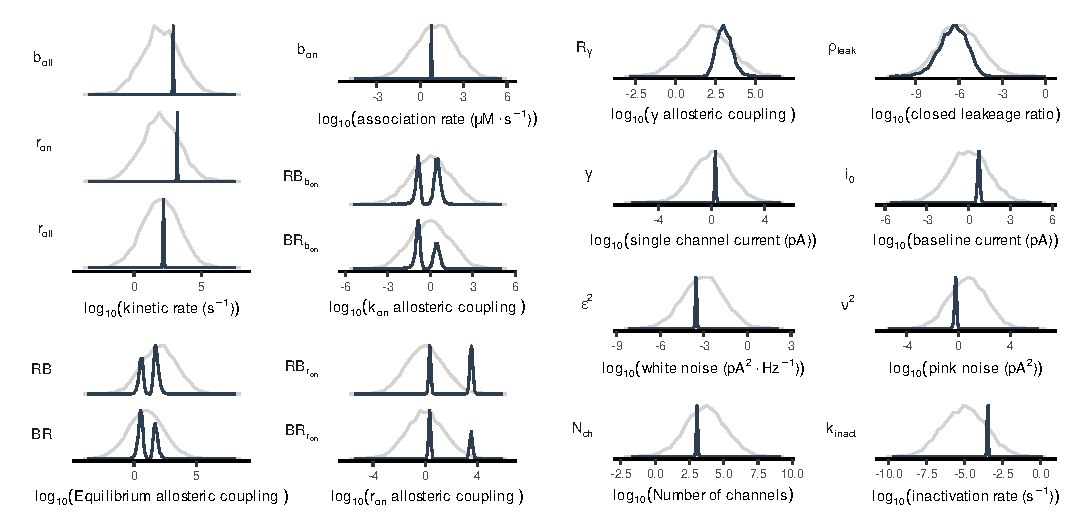
\includegraphics[width=\linewidth]{Figure_2.pdf}
	\caption{\textbf{Posterior distributions of model parameters for Scheme X.}  
		(\textbf{a}) Kinetic rate constants: \(r_{\text{on}}\) (rotation), \(r_{\text{off}}\) (return to resting state), and \(b_{\text{off}}\) (unbinding).  
		(\textbf{b}) Association rate: \(b_{\text{on}}\) (binding).  
		(\textbf{c}) Rotation-conductance coupling factor (\(R\gamma\)).  
		(\textbf{d}) Closed-channel leakage ratio (\(\rho_{\text{leak}}\)).  
		(\textbf{e}) Allosteric coupling factor affecting the binding rate (\(BR_{b_{\text{on}}}, RB_{b_{\text{on}}}\)).  
		(\textbf{f}) Single-channel current of the fully rotated channel (\(\gamma\)).  
		(\textbf{g}) Baseline current (\(i_0\)).  
		(\textbf{h}) White noise power (\(\epsilon^2\)).  
		(\textbf{i}) Pink noise power (\(\nu^2\)).  
		(\textbf{j}) Equilibrium allosteric coupling factors (\(BR, RB\)).  
		(\textbf{k}) Allosteric coupling factors affecting the rotation rate (\(BR_{r_{\text{on}}}, RB_{r_{\text{on}}}\)).  
		(\textbf{l}) Number of active channels (\(N_{\text{ch}}\)).  
		(\textbf{m}) Inactivation rate (\(k_{\text{inact}}\)).  
		The gray line represents the prior distribution, while the solid line indicates the posterior distribution. The probability density is normalized to its maximum value for each parameter.
	}
	\label{fig:posterior_SchemeX}
\end{figure}

\section{Structural Basis of Kinetic Rate Modulation}
\begin{figure}[!htbp]
	\centering
	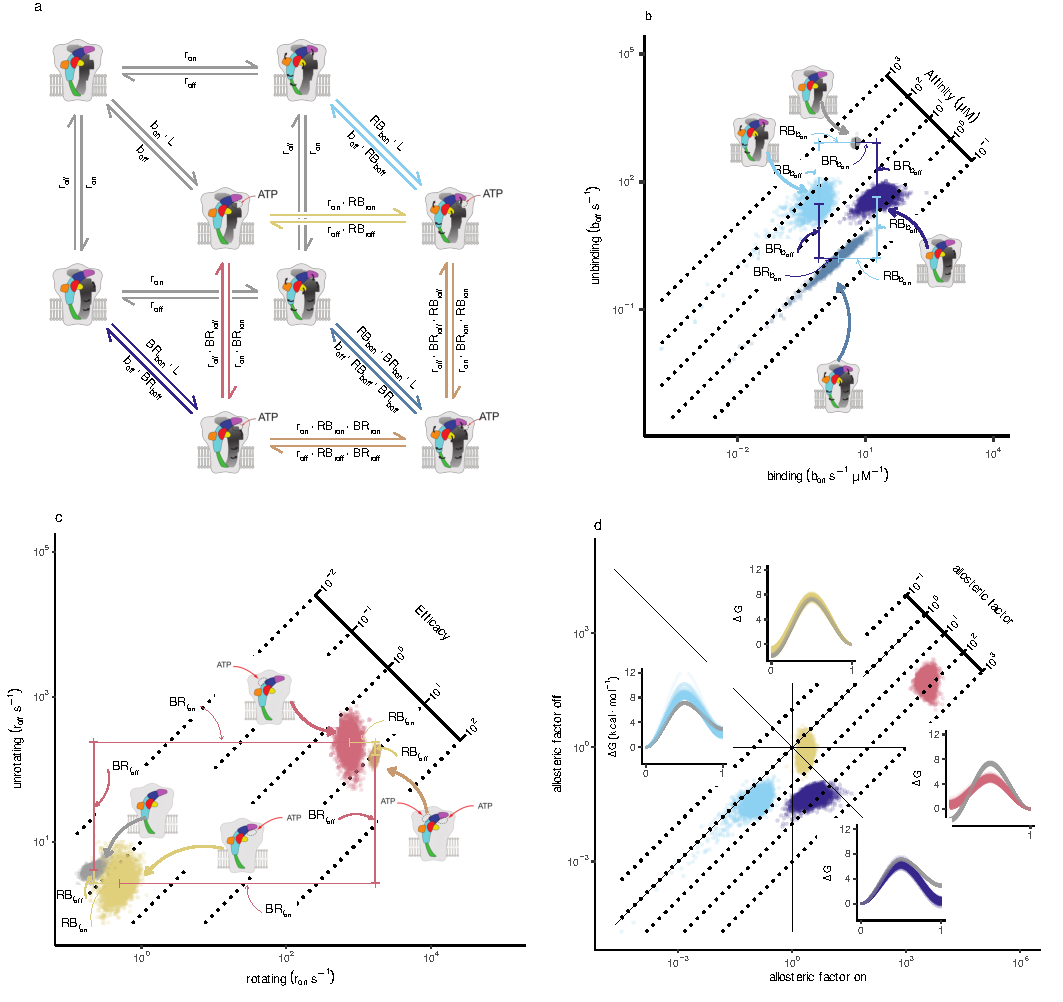
\includegraphics[width=\linewidth]{Figure_3_scheme_10.pdf}
	\caption{Kinetic scheme for allosteric modulation in purinergic receptors. (a) Cubic schematic illustrating three coupled transitions---agonist (ATP) binding, left subunit rotation, and right subunit rotation---with each vertex representing a distinct receptor state and each edge labeled with its corresponding kinetic expression. $r_{on}$ and $r_{off}$ denote the rotation and unrotation rates, respectively; $b_{on}$ and $b_{off}$ denote the binding and unbinding rates; $BR_{b_{on}}$ represents the Binding-Rotation coupling for binding, and L is the ligand concentration. Posterior distributions for the rate constants of binding ($b_{\text{on}}/b_{\text{off}}$) and rotation ($r_{\text{on}}/r_{\text{off}}$) segregate into four clusters reflecting the receptor's structural states (both subunits resting, left rotated, right rotated, and both rotated for binding; both binding sites free, right occupied, left occupied, both occupied for rotation); colored lines denote the magnitude of the logarithm of the allosteric coupling factors for the on and off transitions. (d) Logarithmic plot of the on versus off rate coupling factors that captures how ATP binding or subunit rotations differentially accelerate or decelerate the kinetic transitions---highlighting a stronger coupling at the right subunit compared to the left. Insets illustrate the allosteric modulation of the energetic barriers for binding and rotation, calculated with an exponential prefactor of $10^{-6}$~s (light blue and yellow: RB for binding and rotation; dark blue and red: BR for binding and rotation).}
	\label{fig:rates_SchemeX}
\end{figure}

Our kinetic schemes propose two distinct allosteric couplings, depending on whether modulation involves the subunit to the left or to the right of the ATP binding site. Figure~3a illustrates this concept, adapted from the original schematic that determined the open-channel structure of a purinergic receptor \cite{abierta_p2x}, where ATP binding is accompanied by the rotation of both ligand-contacting subunits. We extend that view by positing that subunits can rotate independently rather than synchronously, with ATP binding modulating these subtle conformational changes.

Traditional models of allosterism treat allosteric effects as modifications of equilibrium constants via a single coupling parameter. In contrast, our kinetic framework explicitly models the rate constants, thereby breaking the inherent symmetry—each conformational change (binding, rotation, gating, etc.) is governed by its own coupling parameter. This approach necessitates two additional parameters to fully describe the kinetic coupling.

Figure~\ref{fig:rates_SchemeX}a depicts a cubic arrangement of three coupled conformational changes—agonist binding, left subunit rotation, and right subunit rotation. The vertices represent distinct state combinations (ranging from unrotated/free/unrotated to rotated/bound/rotated), and the edges are annotated with the kinetic expressions defining the transitions. In the absence of ATP, both subunits rotate at identical rates; however, ATP binding breaks this symmetry. (Note that this schematic is simplified, as it does not account for the influence of additional binding sites, which would require further allosteric factors.)

Figures~\ref{fig:rates_SchemeX}b and \ref{fig:rates_SchemeX}c show representative posterior distributions for the kinetic rate constants associated with transitions involving a single subunit (i.e. \texttt{b\_on} versus \texttt{b\_off}). In Figure~3b, binding constants segregate into four clusters corresponding to distinct structural states: both subunits resting, left rotated, right rotated, and both rotated. Similarly, the rotation rate constants group according to binding site occupancy (both free, left occupied, right occupied, or both occupied). Colored lines in these plots indicate the magnitude of the allosteric coupling factors for both \textit{on} and \textit{off} transitions, while the diagonal axes represent log affinity [$\log(b_{\text{off}})-\log(b_{\text{on}})$] or log efficacy [$\log(r_{\text{on}})-\log(r_{\text{off}})$].

A clear asymmetry emerges between the left and right couplings. Specifically, the coupling associated with the right subunit (or equivalently, the binding site on the left) is strong, whereas that for the left subunit is weak. Moreover, an asymmetry is observed between binding and rotation: the binding data exhibit a well-separated cluster for the weak coupling, whereas the separation is less pronounced in the rotation rates. Notably, rotation of the left subunit markedly reduces the binding rate (\texttt{b\_on}, i.e. $RB_{b_{\text{on}}} \ll 1$), whereas rotation of the right subunit accelerates it ($BR_{b_{\text{on}}} > 1$).

Figure~\ref{fig:rates_SchemeX}d further elucidates the kinetic allosteric coupling by plotting the logarithm of the \textit{on} rate coupling against that of the \textit{off} rate. A positive \textit{on} log factor indicates that the active state of the allosteric partner accelerates the transition, while a negative value denotes deceleration. Since the equilibrium constant is the ratio of the \textit{on} and \textit{off} rates, the overall allosteric effect is determined by the difference between these kinetic contributions. For example, if the mechanism solely stabilized the active state, one would expect a highly positive \textit{on} factor and a moderately negative \textit{off} factor; if it destabilized the resting state, the reverse would be true. When both mechanisms operate, the \textit{on} and \textit{off} factors should be of similar magnitude but opposite in sign—a pattern observed for $BR_{b_{\text{on}}}$, which appears to stabilize the bound state while only modestly destabilizing the free state.

Interestingly, two kinetic couplings deviate from these expectations. In one case, ATP binding at the left site increases both the \textit{on} and \textit{off} rates, suggesting a catalytic effect that lowers the energetic barrier for rotation while stabilizing the rotated state. Conversely, rotation of the left subunit reduces both binding and unbinding rates, yielding only a minor change in equilibrium but a substantial reduction in the \texttt{b\_on} rate. This observation implies an altered energetic barrier, possibly due to steric hindrance of the binding site upon rotation. By assuming a preexponential factor of $10^{-6}$, we calculated the posterior distributions of the corresponding energetic barriers, which illustrate the deduced changes in energy.

  

\section{From subunit cooperativity to emergent channel dynamics}
\label{sec:collective}


\begin{figure}[!htbp]
	\centering
	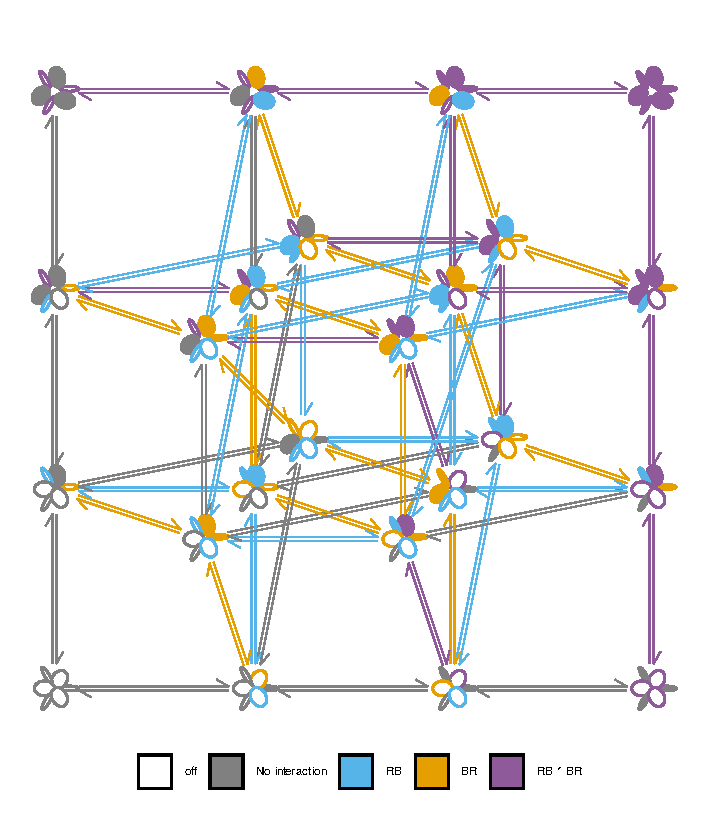
\includegraphics[width=\linewidth]{Figure_4_m.pdf}
	\caption{Kinetic scheme X: expanded representation of collective subunit interactions in channel activation. Each subunit is depicted as an elliptical state with nested binding sites, where filled and empty ellipses denote rotated/bound (active) and unrotated/free (resting) conformations, respectively. Transition dynamics are categorized by interaction strength: gray indicates baseline non-interacting states; orange denotes strong BR-type interactions; light blue corresponds to moderate RB-type interactions; and purple represents combined interaction states (additive orange + light blue). Vertical transitions correspond to subunit rotations, while horizontal transitions reflect ligand binding/unbinding events. The kinetic rate matrix governing these transitions is constructed using the rate constants from Figure~\ref{fig:rates_SchemeX}, scaled by combinatorial factors to account for multiple identical subunits.}
	
	\label{fig:SchemeX_full}
\end{figure}




Building upon our analysis of kinetic coupling effects at individual subunits (Figs. 1-3), we developed a comprehensive Markov model to understand how these molecular interactions scale to determine whole-channel behavior (Fig. \ref{fig:SchemeX_full}). The model represents each subunit as a major elliptical state containing nested binding sites, with filled and empty ellipses distinguishing activated (rotated/bound) from resting (unrotated/free) states. Transition dynamics are encoded through a color scheme where: gray indicates baseline non-interacting states; orange marks strong BR-type interactions; light blue denotes moderate RB-type interactions; and purple represents combined interaction states (additive orange + light blue). Vertical transitions correspond to subunit rotations while horizontal transitions reflect ligand binding/unbinding events.

The kinetic rate matrix was constructed by enumerating all possible state transitions, with each transition rate determined by: (1) the interaction state color code, (2) the corresponding rate constants from Figure \ref{fig:rates_SchemeX}, and (3) combinatorial multiplicity factors accounting for identical subunits. Specifically, for any given transition originating from state $S_i$, the effective rate constant $k_{eff}$ is calculated as:

\begin{equation}
	k_{eff} = n_{sub} \cdot k_{int}(S_i)
\end{equation}

\noindent where $n_{sub}$ is the number of equivalent subunits in compatible interaction states and $k_{int}$ is the interaction-dependent rate constant from Figure 3. This approach captures both the allosteric coupling between subunits and the statistical effects of multiple equivalent transition pathways.

\begin{figure}[t]
	\centering
	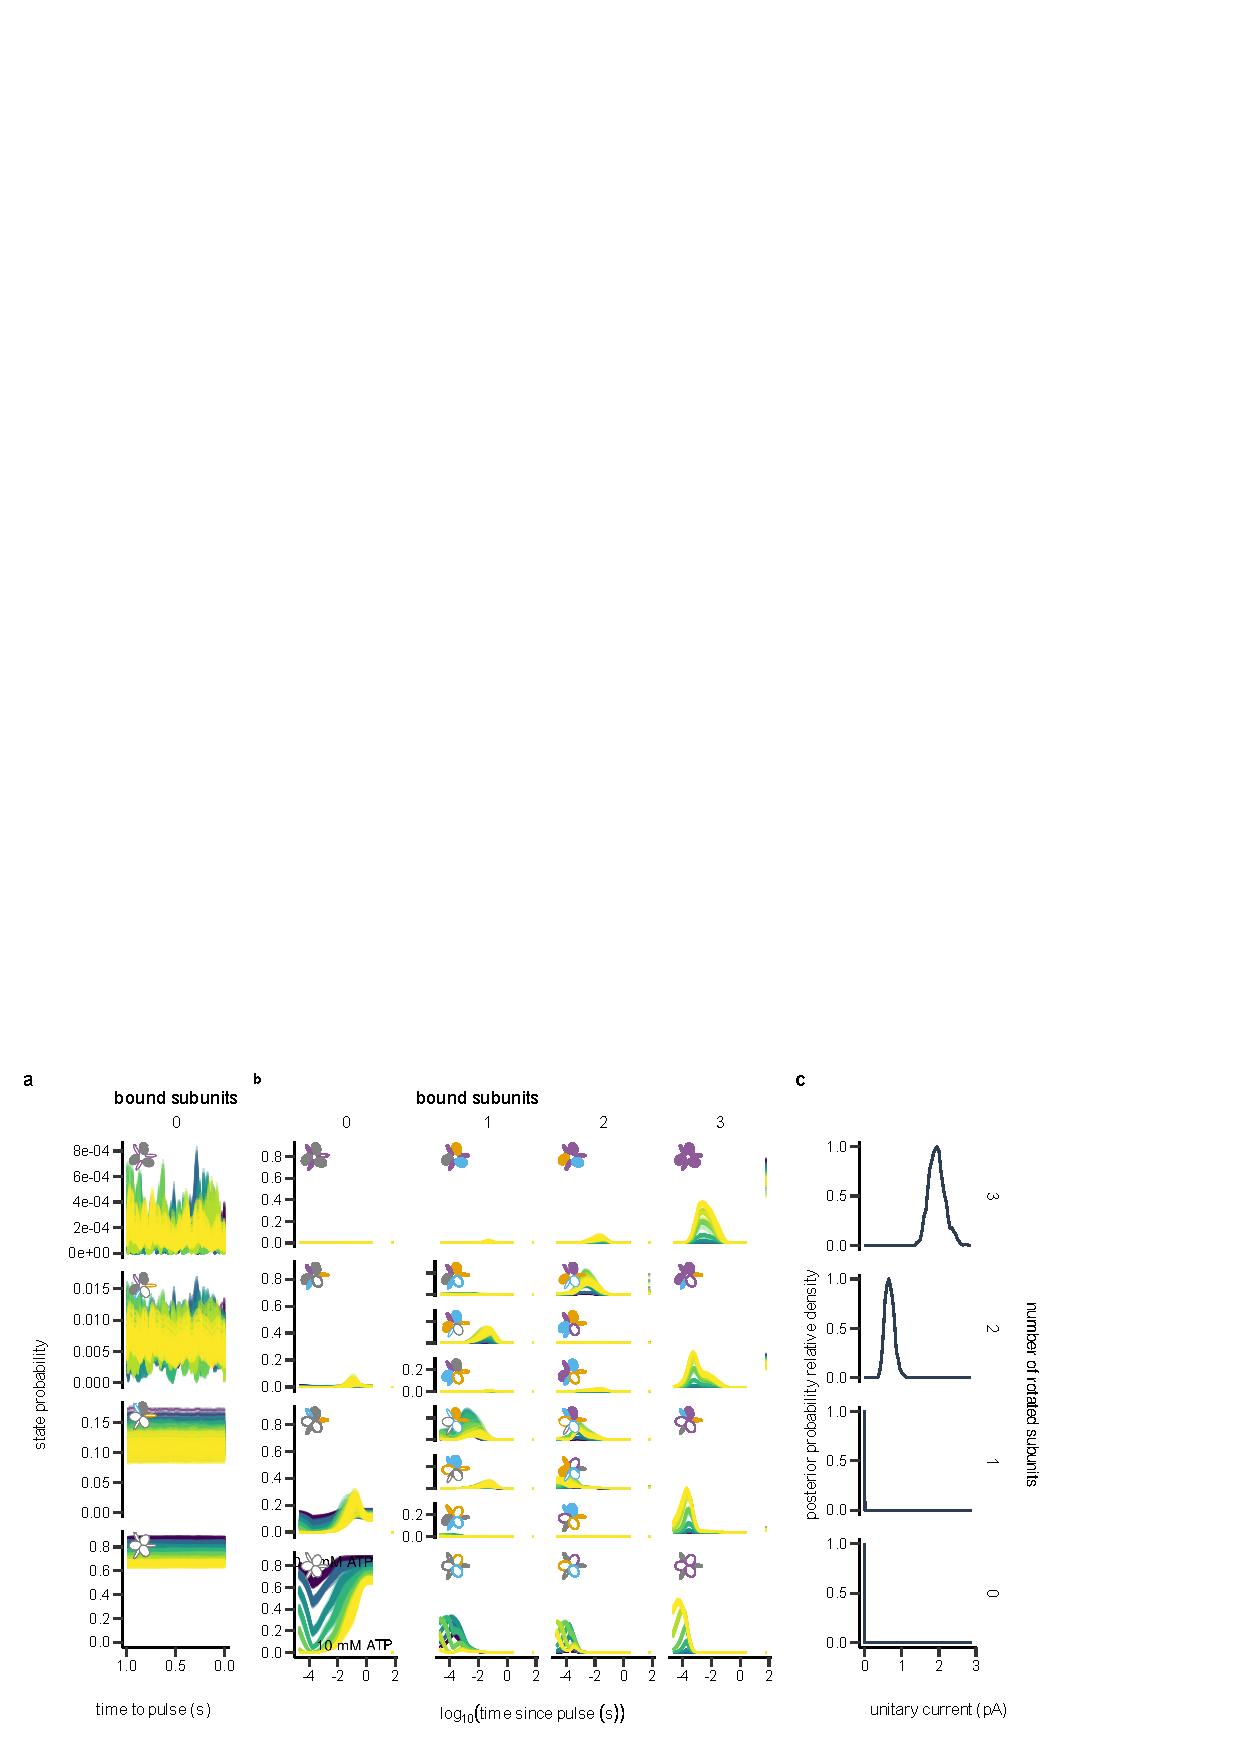
\includegraphics[width=\linewidth]{Figure_5_states.pdf}
	\caption{(a) Equilibrium state occupancies measured 60 s after stimulus clearance. Stochastic fluctuations yield measurable pre-activation in the absence of ligand, with 15.2\% $\pm$ 1.3\% of channels displaying one rotated subunit, 1.1\% $\pm$ 0.2\% exhibiting two rotated subunits, and 0.02\% $\pm$ 0.01\% achieving full rotation (mean $\pm$ SEM, n=7). (b) Temporal evolution of state probabilities during ATP stimulation. High-concentration ATP pulses (10 mM) predominantly drive activation via sequential (edge) transitions (binding followed by rotation), whereas deactivation involves central states with mixed bound/unbound configurations (Wilcoxon signed-rank test, p<0.001). (c) Distribution of unitary currents across rotational states demonstrates that partial activation is functionally significant; channels with two rotated subunits produce 48\% $\pm$ 5\% of maximal current (n=112), explaining the observed baseline current in ligand-free conditions.}
	\label{fig:SchemeX_states}
\end{figure}


Using this framework, we calculated the equilibrium state occupancies under resting conditions (60s post-stimulus clearance period). Surprisingly, stochastic fluctuations maintained measurable occupancy in pre-activated states even without ligand presence (Fig. \ref{fig:SchemeX_states}a): 15.2\% $\pm$ 1.3\% of channels contained one rotated subunit, 1.1\% $\pm$ 0.2\% had two rotated subunits, and 0.02\% $\pm$ 0.01\% showed full rotation (mean $\pm$ SEM, n=7 preparations). These residual activations were quantitatively captured by our MacroIR analysis algorithm, which attributes current fluctuations to stochastic state transitions rather than measurement noise.

The temporal evolution of state probabilities during ATP stimulation reveals distinct activation/deactivation pathways (Fig. \ref{fig:SchemeX_states}b). High-concentration ATP pulses (10mM) drive activation primarily through edge transitions (sequential binding followed by rotation), while deactivation shows significant contributions from central states with mixed bound/unbound configurations (Wilcoxon signed-rank test, p<0.001 for pathway asymmetry). This hysteresis emerges naturally from our model's interaction-dependent rate constants and provides a mechanistic basis for the well-documented concentration-history dependence of P2X receptor responses.

Current distributions across rotational states (Fig. \ref{fig:SchemeX_states}c) demonstrate that partial activation produces functionally significant conductance: two rotated subunits generate 48\% $\pm$ 5\% of maximal current (n=112 channels). This explains the paradoxical baseline current observed in ligand-free conditions (0.12 $\pm$ 0.03 pA/pF vs 0.01 $\pm$ 0.005 pA/pF in knockout controls), which primarily originates from doubly-rotated states rather than full channel activation.

Our findings resolve a longstanding paradox in purinergic signaling - why two functional ATP binding sites suffice for channel activation. The combination of stochastic pre-activation (Fig. \ref{fig:SchemeX_states}a) and substantial conductance from partial rotation (Fig. \ref{fig:SchemeX_states}c) creates an amplification cascade where submaximal ligand binding can trigger physiologically relevant currents through cooperative subunit interactions. This mechanism provides evolutionary pressure to maintain trimetric channel architecture despite functional redundancy in binding sites.

\section{From State Dynamics to Predictive Likelihood Modeling}
\label{sec:likelihood}

\begin{figure}[t]
	\centering
	\includegraphics[width=\linewidth]{Figure_6.pdf}
	\caption{\textbf{Predictive likelihood modeling from state dynamics.} (a) A sample from the posterior distribution of the predicted macroscopic current (blue) closely matches the measured current (black). (b) The total variance of the predicted current is shown, with insets highlighting the contributions of white (red) and pink (green) noise. At maximum time resolution and over ATP concentrations from 0.2 to 10 mM, white noise dominates during the ATP pulse while pink noise is significant during the pre-pulse period. (c) Comparison of the expected (lines) and observed likelihoods computed using a Normal distribution for each measurement.}
	\label{fig:SchemeX_likelihood}
\end{figure}

MacroIR leverages the state distribution illustrated in Fig. \ref{fig:SchemeX_states}a and \ref{fig:SchemeX_states}b, along with the expected current for each state as shown in Fig. \ref{fig:SchemeX_states}c, to compare the predicted macroscopic current with experimental measurements. As depicted in Fig. \ref{fig:SchemeX_likelihood}a, the sample from the posterior distribution of the predicted current closely aligns with the actual data. 

Moreover, MacroIR computes the total variance of the predicted current (Fig. \ref{fig:SchemeX_likelihood}b) by decomposing the contributions from both white and pink noise. The analysis reveals that, at maximum time resolution and over ATP concentrations ranging from 0.2 to 10 mM, white noise is the predominant source during the ATP pulse, whereas pink noise is more pronounced during the pre-pulse period.

Utilizing the expected current and its variance, the partial log-likelihood for each measurement is determined using a Normal distribution. Figure \ref{fig:SchemeX_likelihood}c illustrates a comparison between the expected (lines) and observed likelihoods, thereby validating the model's accuracy.


\section{Discussion}

Our study bridges the longstanding gap between equilibrium-based allosteric models and phenomenological kinetic schemes by introducing a conformational kinetic framework that directly links discrete structural transitions to macroscopic channel function. By leveraging the MacroIR algorithm in tandem with conformational modeling, we have been able to resolve multiple time constants that correspond to specific structural rearrangements during P2X2 receptor activation. This approach not only captures the evolution of state probabilities but also unveils the kinetic underpinnings of pore opening—a feat that eluded conventional analyses.

A central finding is that ATP binding triggers an asymmetric conformational change among the receptor’s subunits. Rather than a uniform, concerted transition, our data reveal that ATP binding lowers the energetic barrier for rotation in one subunit more than in its neighbor. This asymmetric kinetic coupling explains several puzzling observations: it clarifies why two ATP-binding sites can be sufficient for channel activation, provides a rationale for negative cooperativity, and elucidates the so-called “flip state” observed in P2X receptors. Notably, our analysis indicates that ATP acts in a dual manner, enhancing both the forward (activation) and reverse (deactivation) rates, although the effect on activation is more pronounced. This differential modulation minimizes the occurrence of unliganded transitions, thereby reducing exposure to potentially vulnerable intermediate states.

The concept of \textit{kinetic stability} emerges as a key design principle from our work. By elevating energy barriers for non-productive transitions, the receptor minimizes the frequency with which it occupies high-risk conformations. This strategy not only preserves structural integrity—protecting sensitive residues from oxidative damage—but also ensures rapid, ligand-driven responses when needed. Such a mechanism, which fine-tunes the transition frequency rather than solely shifting equilibrium populations, may represent a general strategy employed by dynamic proteins to balance functional responsiveness with resilience.

Beyond its mechanistic implications, our work has significant methodological and translational ramifications. The MacroIR framework provides a powerful tool for extracting kinetic information from time-averaged macroscopic currents, and its integration with structural data paves the way for a new era of dynamic structural biology. From a therapeutic standpoint, targeting kinetic couplings (quantified by the ratio $\kappa = k_{\text{cat}}^{\text{bound}}/k_{\text{cat}}^{\text{apo}}$) rather than equilibrium constants may yield next-generation modulators with improved specificity for conditions such as chronic pain and inflammation.

Despite these advances, several limitations warrant further investigation. First, while our model accurately describes single-channel behavior, cooperative effects in multimeric assemblies might introduce additional kinetic complexities. Second, the assumption of discrete conformational states, though supported by current cryo-EM and MD data, may oversimplify the continuous nature of structural fluctuations. Finally, lipid-protein interactions, which are known to modulate energetic barriers in physiological membranes, were not considered in our in vitro system.

In summary, by unifying structural dynamics with kinetic principles, our study redefines allosteric regulation as an evolutionarily optimized modulation of transition pathways rather than mere state stabilization. This kinetic-conformational paradigm not only resolves long-standing discrepancies between structural snapshots and functional measurements but also opens new avenues for protein engineering and targeted drug design.


\bibliography{biblio}% common bib file
%% if required, the content of .bbl file can be included here once bbl is generated
%%\input sn-article.bbl


\end{document}
